%!TEX root = Thesis.tex

\chapter{Experimental Results}\label{cha:experimental_results}     Throughout
the course of development of the full framework that we present in this
thesis, we make extensive use of three components: visual car detection,
environment modeling and planning.

\section{Visual Car Detection}\label{sec:visual_car_detection}
\begin{figure}[p]%
\centering
\subfloat{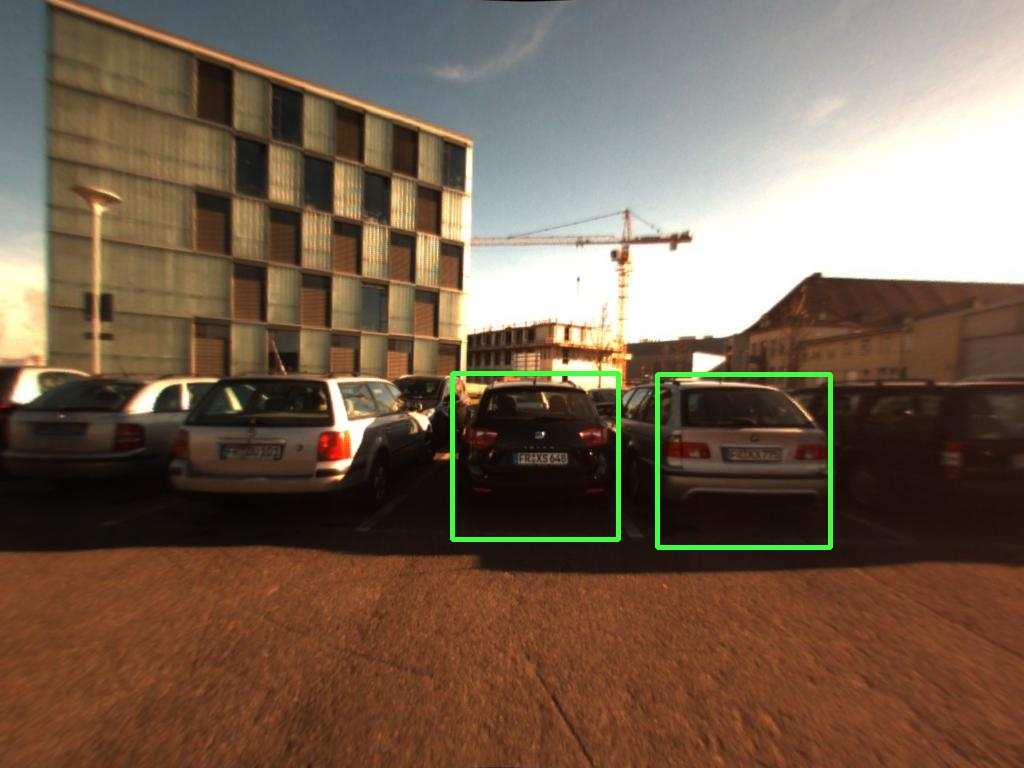
\includegraphics[width=0.35\textwidth]{pictures/det_1.jpg}}
\subfloat{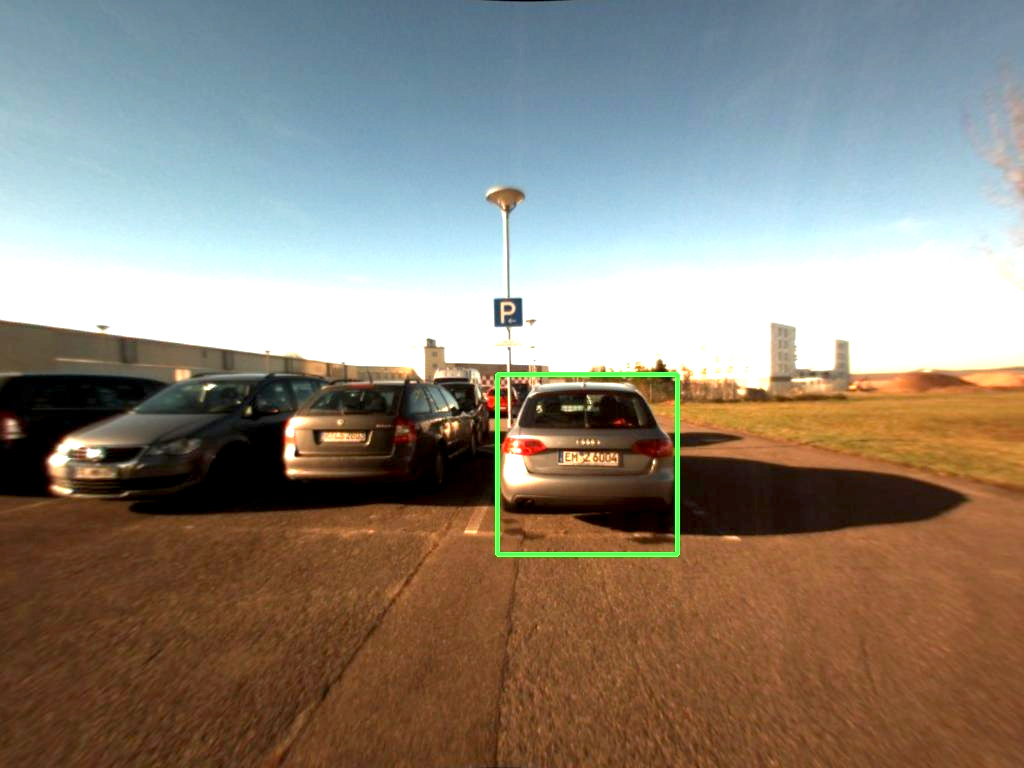
\includegraphics[width=0.35\textwidth]{pictures/det_2.jpg}}
\subfloat{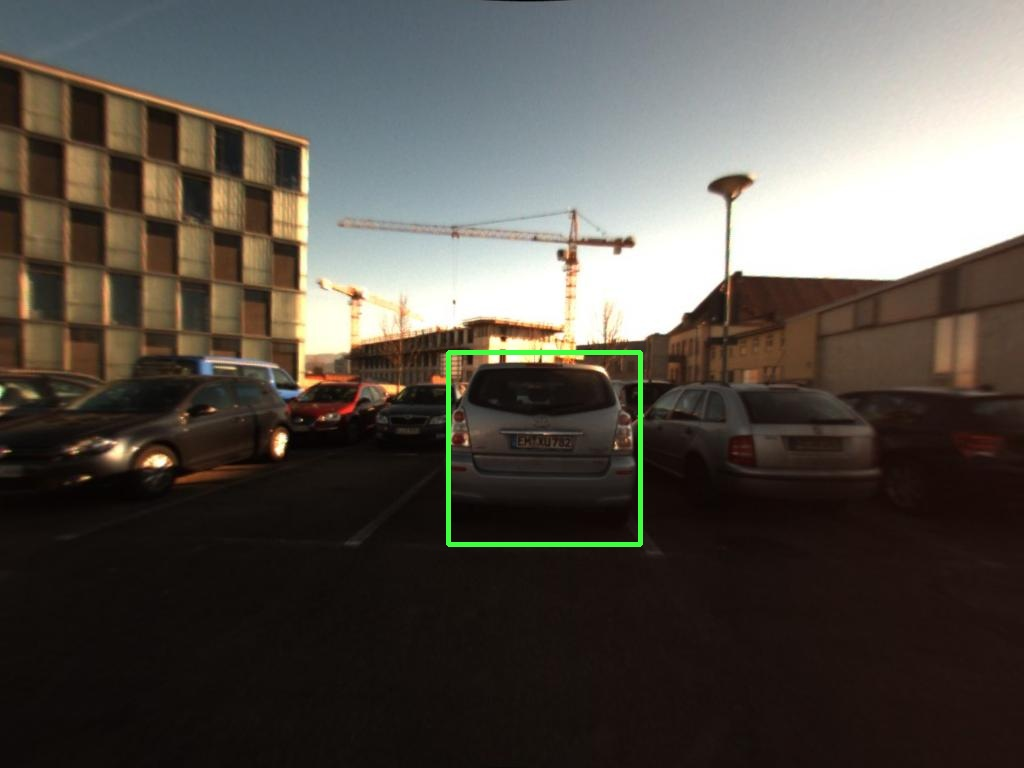
\includegraphics[width=0.35\textwidth]{pictures/det_3.jpg}}\\
\subfloat{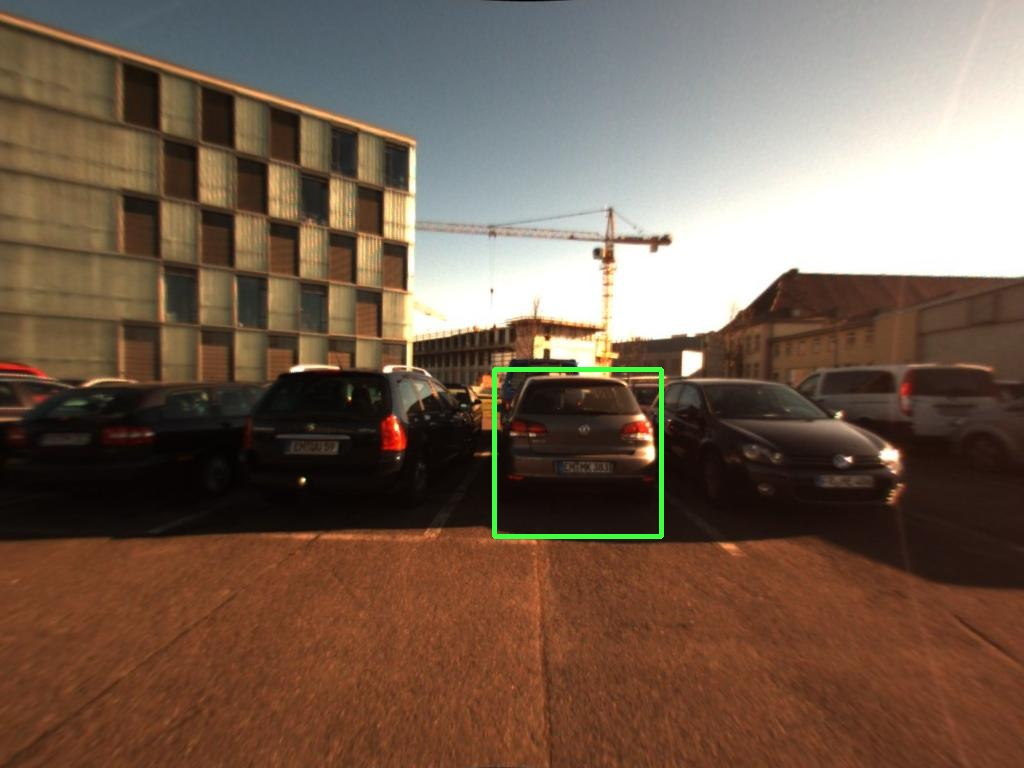
\includegraphics[width=0.35\textwidth]{pictures/det_4.jpg}}
\subfloat{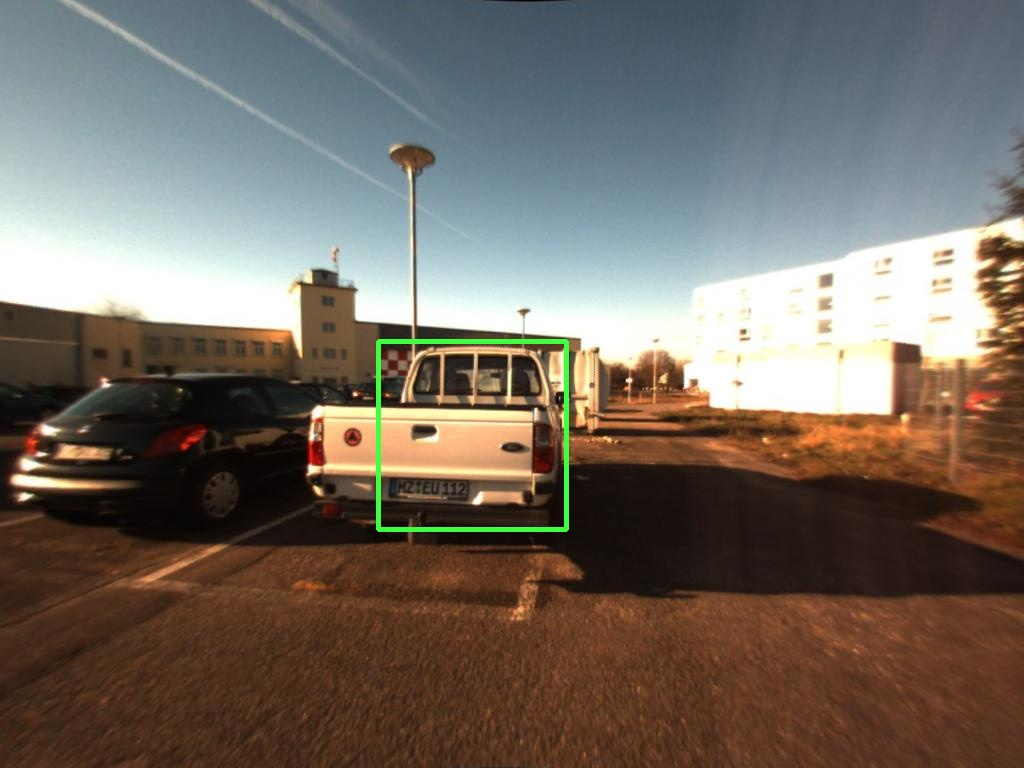
\includegraphics[width=0.35\textwidth]{pictures/det_5.jpg}}
\subfloat{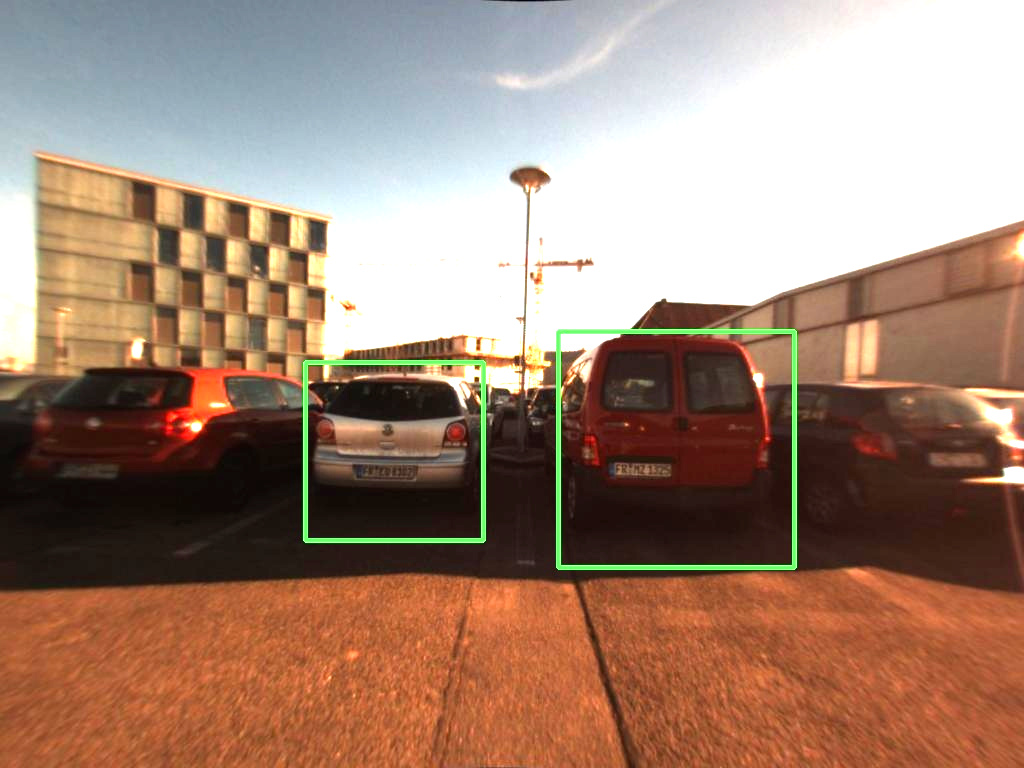
\includegraphics[width=0.35\textwidth]{pictures/det_6.jpg}}\\
\subfloat{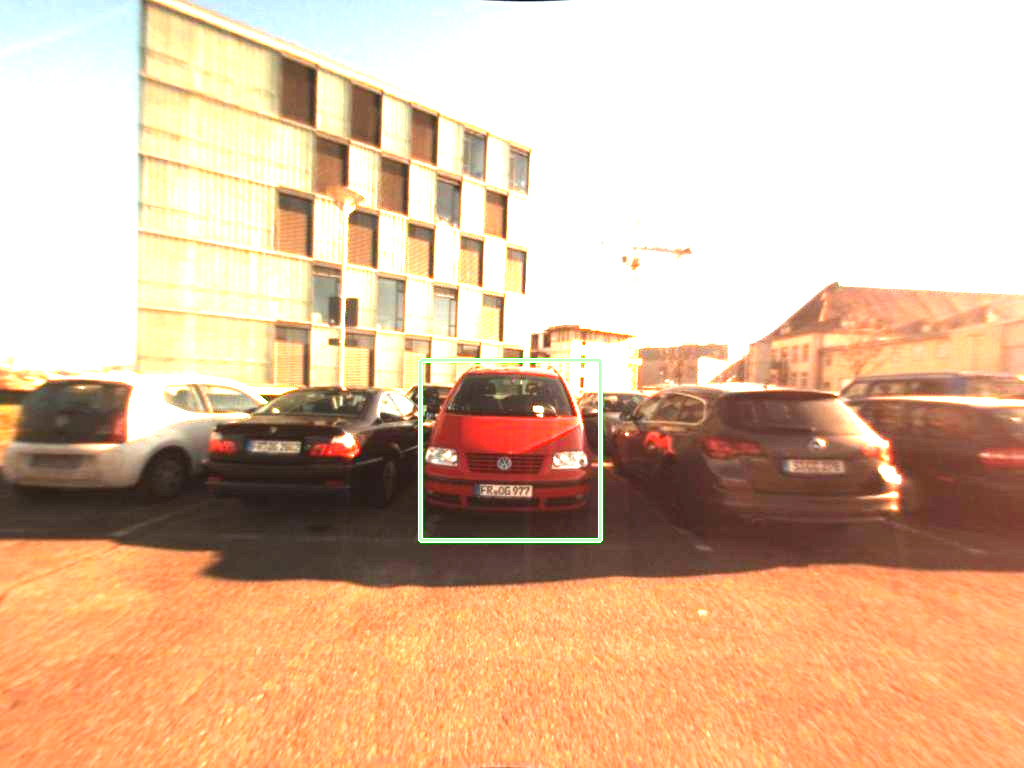
\includegraphics[width=0.35\textwidth]{pictures/det_7.jpg}}
\subfloat{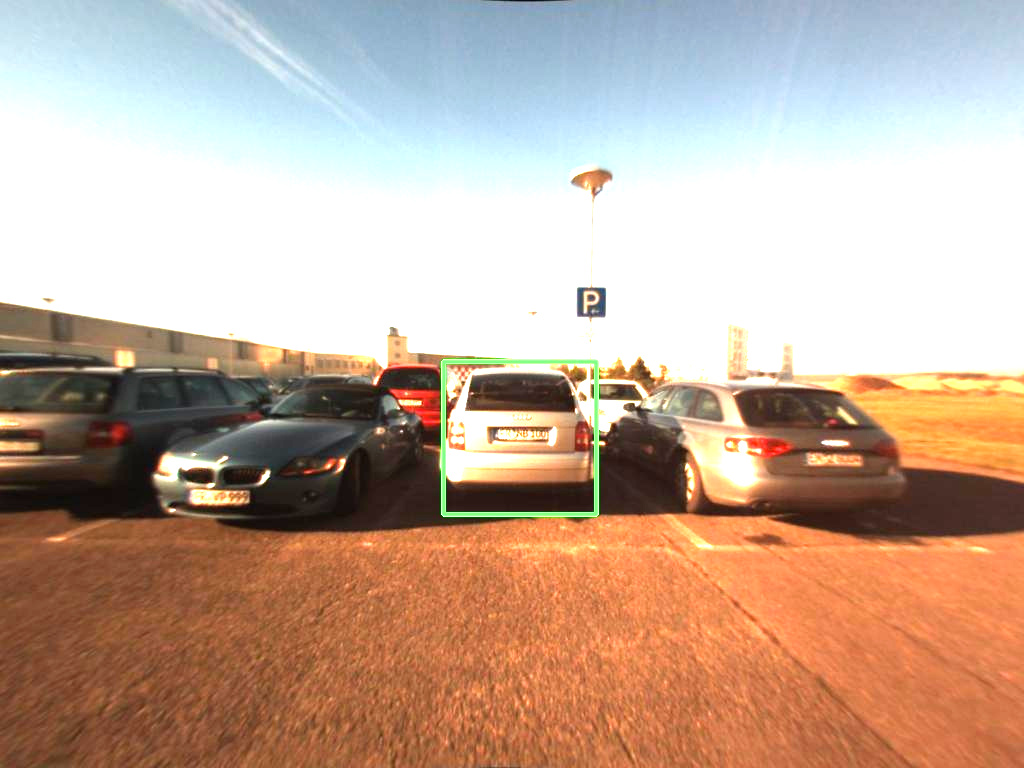
\includegraphics[width=0.35\textwidth]{pictures/det_8.jpg}}
\subfloat{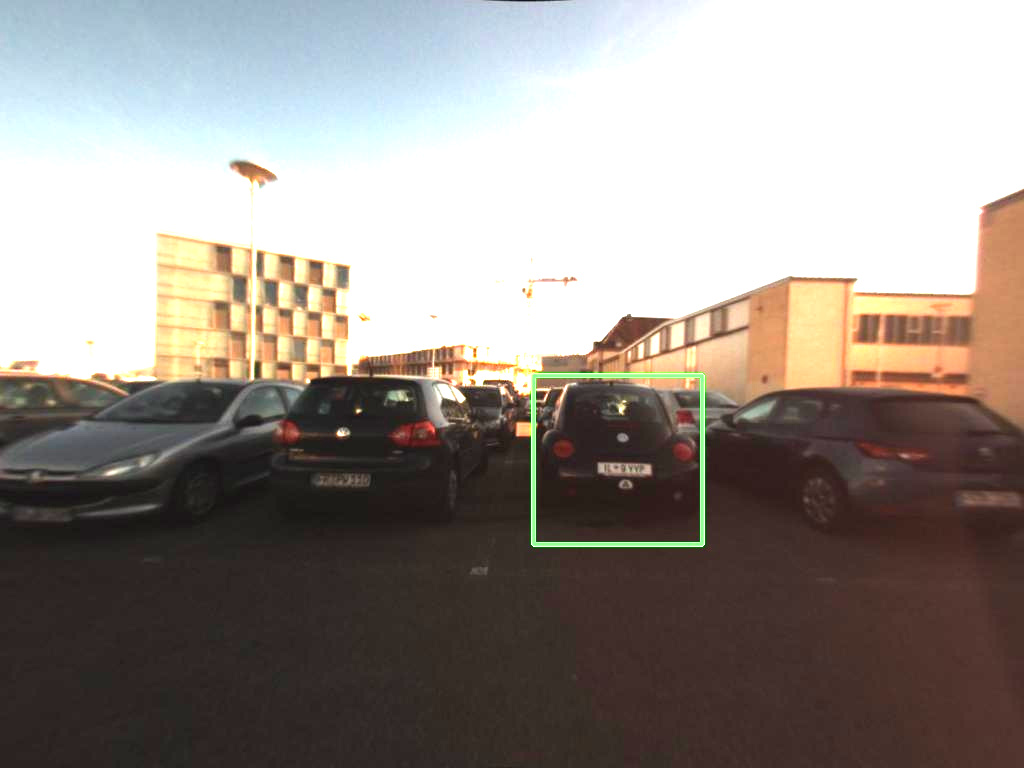
\includegraphics[width=0.35\textwidth]{pictures/det_9.jpg}}\\
\subfloat{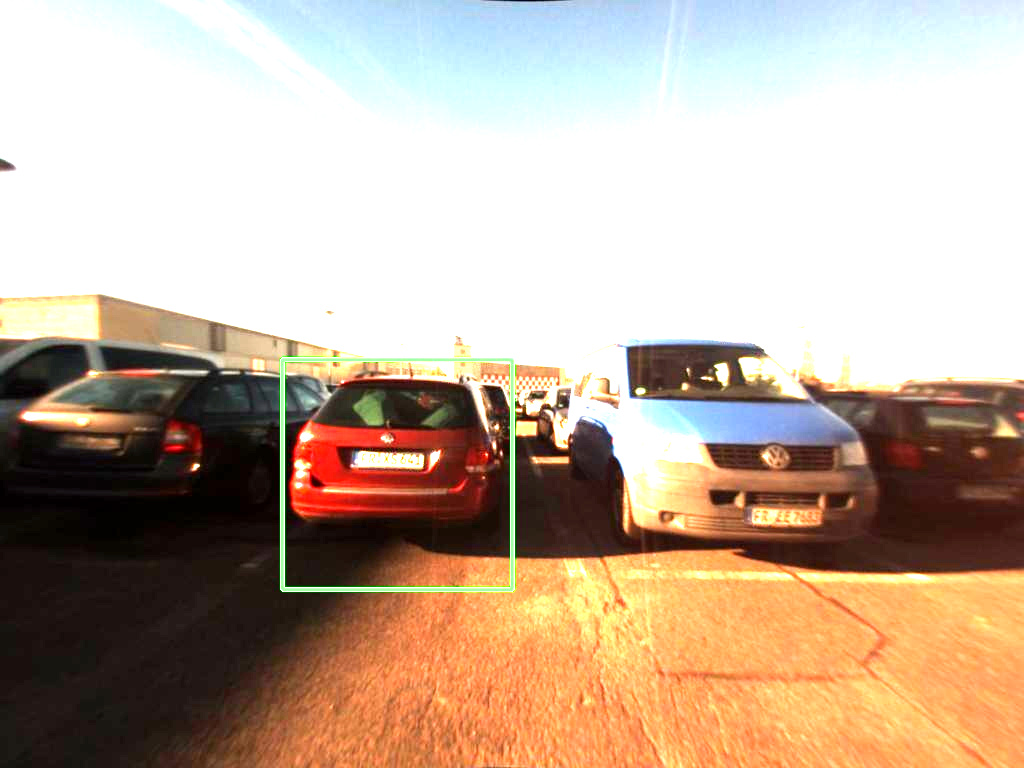
\includegraphics[width=0.35\textwidth]{pictures/det_10.jpg}}
\subfloat{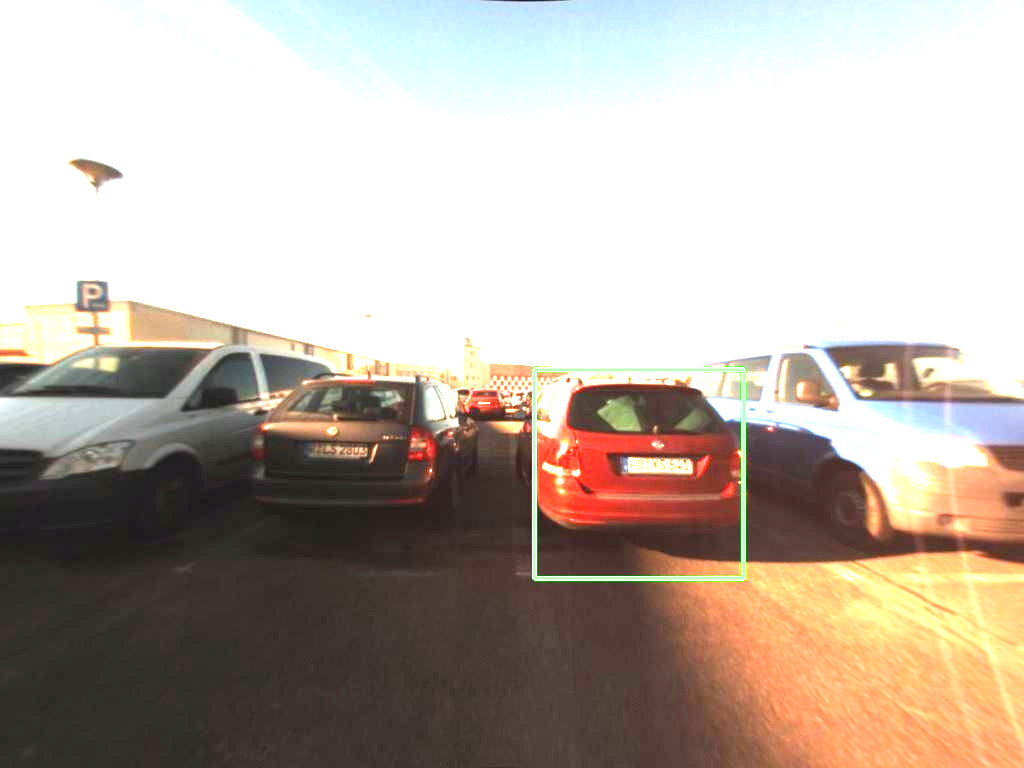
\includegraphics[width=0.35\textwidth]{pictures/det_11.jpg}}
\subfloat{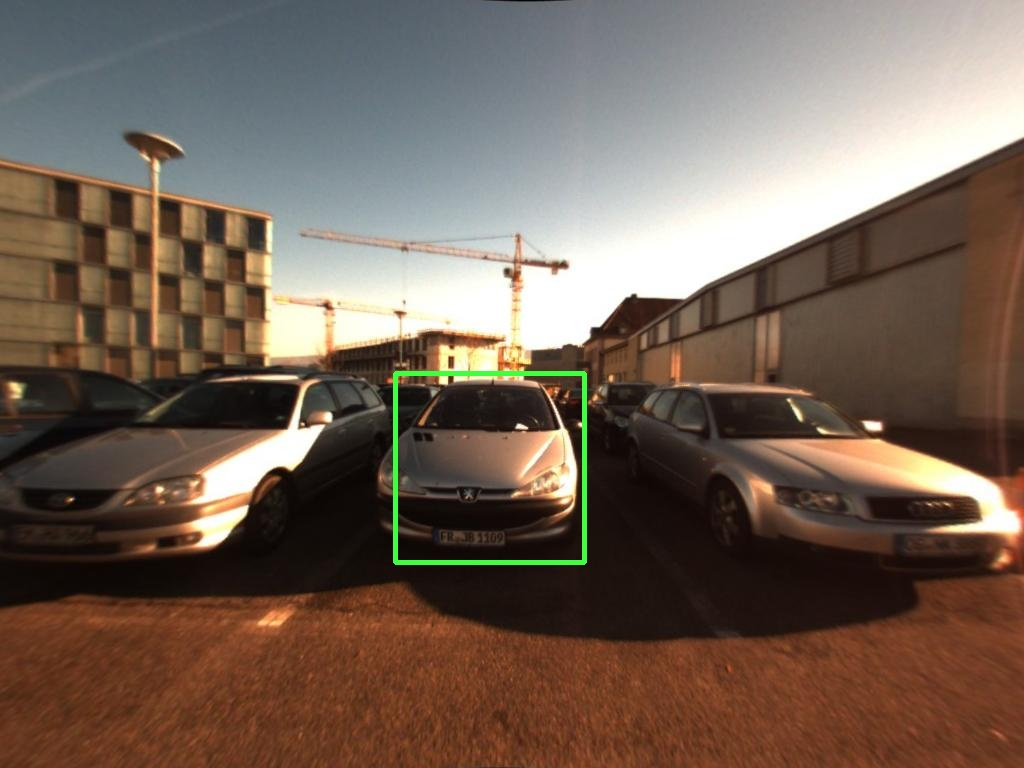
\includegraphics[width=0.35\textwidth]{pictures/det_12.jpg}}\\
\caption{Examples of detections of different cars under different light conditions.}
\label{fig:detection_examples}
\end{figure}

This experimented is carried out in order to show the detection rate of visual
detection utilizing the HOG features.

We create a training dataset that contains positive and negative examples that
can be fully described with a HOG descriptor in order to cluster the outcome
via SVM later. The cars don't look the same from different views, wherefore we
have positive training data for different angles of the cars. We have
considered to create training samples for four different views of the cars ---
front, back and both left and right sides.

The sides of the car are invariant under the mirror transformation. Front and
back of the car, though different to human point of view, seem to be similar
in the HOG visualization. Therefore, the corresponding datasets can be
combined into one.

The positive dataset was filled from different sources, INRIA Car Dataset
by~\cite{inriadata}, Motorway Car Dataset by~\cite{TMEMotorwayDataset} and
images found in a public domain via Google.

Let us explain in more detail the experiments on the front/rear detection. The
side detection can be handled in a similar way. The final positive training
dataset contains 440 images, $128 \times 128$ pixels each. Each of those
images contains only a car and can be fully described with a HOG descriptor.
The negative set is created in the way described in the work
of~\cite{dalal2005}. First, a number of $128 \times 128$ pixels patches is
sampled from the images, that contain no cars. This data is then used as the
negative data for the classifier training process. The false detections of the
outcome are also put to the same negative training set. This is performed
several times. The final negative dataset contains 7972 images, each of which
is $128 \times 128$ pixels big. The system shows the performance of \todo{add
detection rate for my approach} in detecting the cars the camera faces. Some
of the detection examples are presented in
Figure~\ref{fig:detection_examples}.

% section visual_car_detection (end)

\section{Occupancy Modeling}\label{sec:occupancy_modeling}
We here present the examples of occupancy data aggregated to the occupancy grids as well as into the pre-defined parking lot positions. The occupancy data is based on the 2D data obtained with lasers, mounted on the robot. \todo{do a photo of the robot with a camera} As can be seen in the figure, the stereo camera is mounted on the same z-axis as the laser range finder. We search for the needed endpoints that represent the cars as described in chapter \nameref{cha:our_approach}, section \nameref{sec:perception}
The precision of car position modeling can be seen in the figure. \todo{what to write more???}
% section occupancy_modeling (end)

\section{Planning}\label{sec:planning}
As can be seen in the previous section, the question of how to use the occupancy grids in order to build a planner on top of the occupancy information in them is still open. We thus currently focus on a planner based upon the pre-defined parking lots positions. However, the planner itself is generic, which allows to use it in any situation alike. For now we can manipulate the constant time for taking the next action. It can be seen, that if this value is set to a very big value, the optimal action for each state is to park right there just to keep the overall reward positive. If we on the contrary set this constant to 0, the optimal decision will be to move around the parking lot until we have found the best (closest to the goal) parking lot and then try to park there.
The most optimal result is achieved if the cost of moving between the parking lots by car is the distance between them, divided by the speed of the car. This makes the algorithms consider a trade-off between shorter routes while searching for a place and better parking lots, situated closer to the goal, weighted by the occupancy probability.
The next example shows the behavior of the agent under different current occupancy.
% section planning (end)
% chapter experimental_results (end)
